A metodologia do trabalho foi baseada nas etapas do processo de descoberta de conhecimento em base de dados (\textit{Knowledge Discovery in Databases} - KDD)\cite{KDD}, aplicada a um conjunto de dados textuais. As atividades foram divididas em 4 etapas principais: Coleta de Dados, Técnicas de Pré Processamento, Mineração de Dados e Avaliação do Modelo. 

\section{Coleta de Dados}

\subsection{Artigos}
A coleta de artigos na Interface de Programação de Aplicações (API) do \textit{PubMed}\footnote{\url{https://pubmed.ncbi.nlm.nih.gov}} foi realizada por meio de duas abordagens: a primeira utilizou palavras-chave para obter uma lista de identificadores de artigos relacionados ao domínio de interesse, a segunda acessou cada artigo individualmente para extrair as informações relevantes. Entre os dados coletados estão: Identificador Digital de Objetos (DOI), Informações Pessoais Identificáveis (PII), Localizador Uniforme de Recursos (URL), periódico (\textit{Journal}), título, resumo (\textit{Abstract}), autores, ano de publicação e palavras-chave associadas ao texto.

Esse processo foi conduzido por meio de um coletor automatizado, implementado para realizar consultas à API com termos específicos, incluindo \textit{dairy, dairy cows, dairy farming, dairies}, não se limitando a esses exemplos. Os artigos recuperados tiveram seus títulos e resumos extraídos e armazenados em formato estruturado, compondo uma base de dados destinada à etapa de pré-processamento. O conjunto final inclui periódicos relevantes, como o \textit{Journal of Dairy Science}, que aborda aspectos técnicos e científicos voltados ao aumento da produtividade e ao bem-estar do gado leiteiro.

\subsection{Perguntas e Respostas sobre a Pecuária Leiteira}
O segundo estágio do trabalho consistiu na extração de 500 perguntas e respostas sobre gado leiteiro de \citeonline{embrapa2012gadoleite}, utilizado como referência para a avaliação das respostas geradas pelos modelos. Para cada pergunta, a resposta do modelo será comparada com a resposta de referência do livro, permitindo medir a similaridade semântica e léxica. Para isso, realizou-se um pré-processamento do texto, convertendo o conteúdo do PDF para formato textual por meio da biblioteca \textit{PyPDF}\footnote{\url{https://pypi.org/project/PyPDF2}} do Python.

\section{Pré-Processamento e Transformação}

As técnicas de pré-processamento tiveram como objetivo assegurar a qualidade e a consistência da base construída. Inicialmente, foram removidos registros duplicados e valores nulos, evitando redundâncias que poderiam comprometer os resultados.

Para os artigos coletados via API, realizou-se a extração dos identificadores textuais presentes nas respostas, selecionando apenas as informações relevantes. A Figura \ref{fig:art_pubmed} apresenta um exemplo do retorno de um artigo pela API. Esses dados foram então armazenados em formato CSV, facilitando o manuseio e a utilização nas etapas seguintes,  conforme representado na Tabela \ref{tab:exemplo_art_csv}.



\begin{figure}[H]
\centering
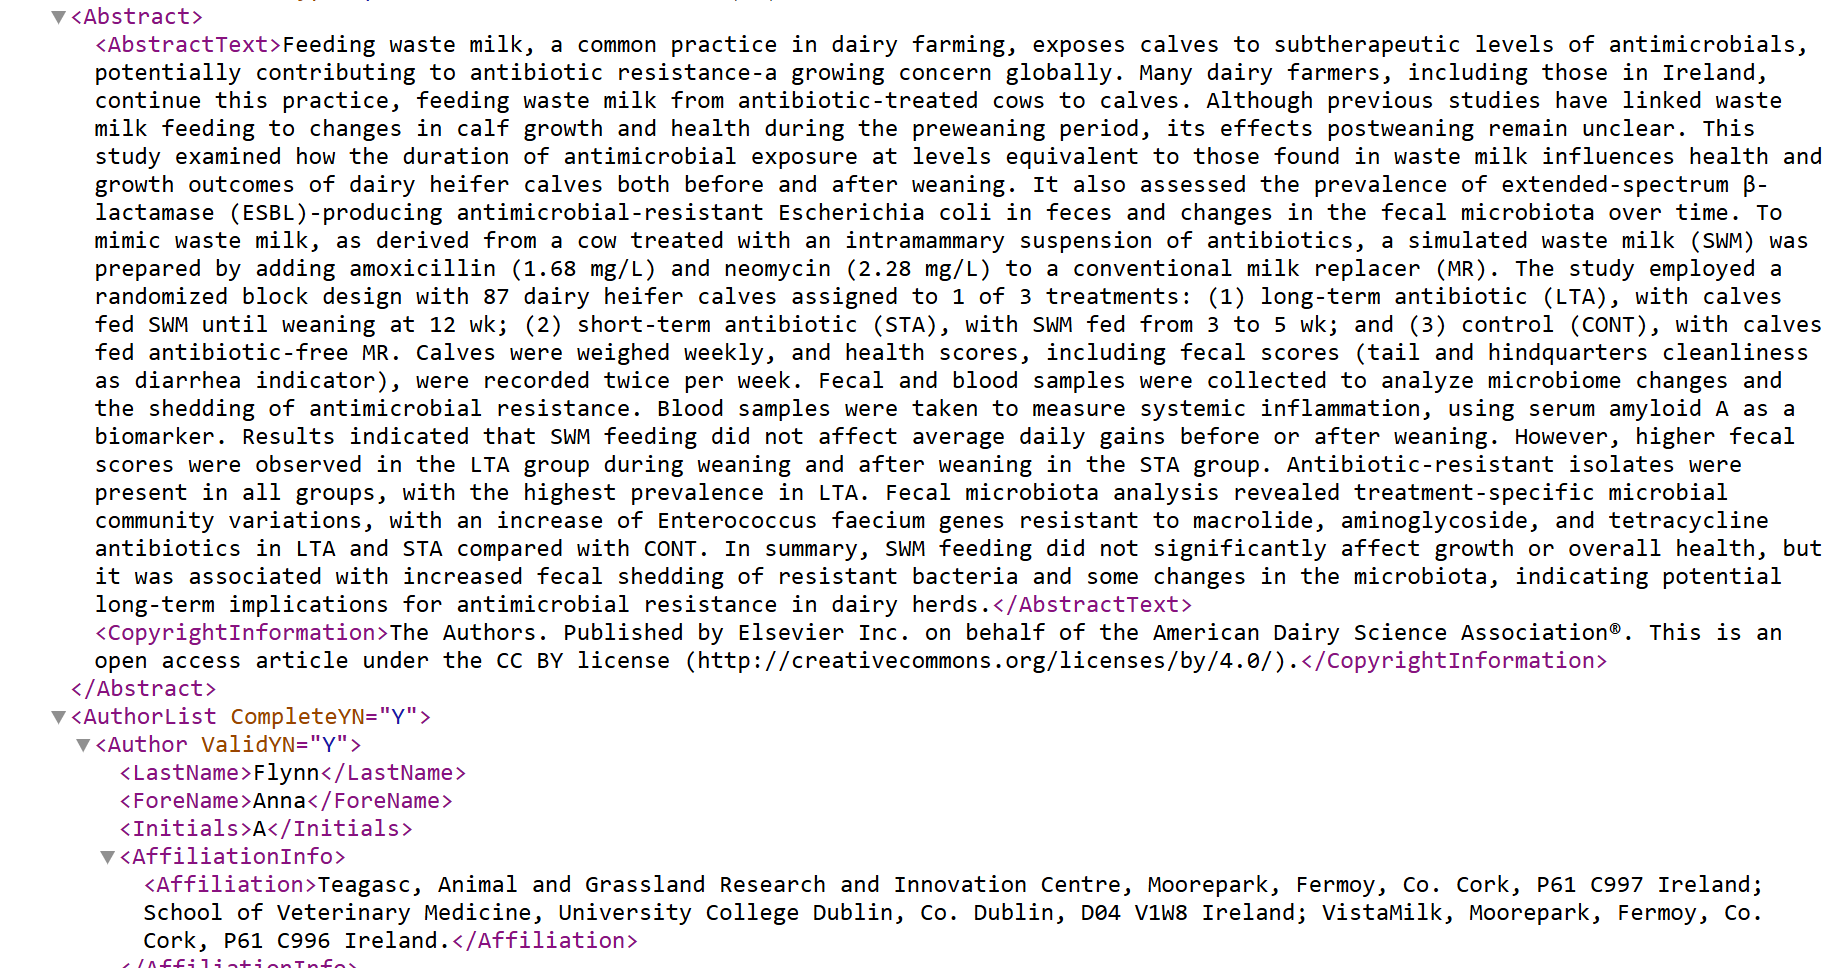
\includegraphics[width=0.95\linewidth, height=0.8\textheight, keepaspectratio]{imagens/art_pubmed1.png}
\caption{Artigo retornado pela API. Fonte: \cite{PubMed}}
\label{fig:art_pubmed}
\end{figure}


\begin{table}[H]
    \centering
    \resizebox{\textwidth}{!}{
        \begin{tabular}{c|p{2.5cm}|p{2.5cm}|p{3.5cm}|p{5cm}|p{3.5cm}}
             PubMedID & URL & JOURNAL & Title & Abstract & Keywords \\
             \midrule
             40383390 & \url{https://eutils.ncbi.nlm.nih.gov/entrez/eutils/efetch.fcgi?api_key={apikey}&db=pubmed&rettype=abstract&id=40383390} & Journal of Dairy Science & Effects of feeding a simulated waste milk on growth, health, fecal microbiota, and antibiotic resistance in dairy heifer calves. & Feeding waste milk, a common practice in dairy farming, exposes calves to subtherapeutic levels of antimicrobials, potentially contributing to antibiotic resistance... &
             antibiotic, average daily gain, microbiota, waste milk
        \end{tabular}
    }
    \caption{Exemplo de registro de artigo em CSV.}
    \label{tab:exemplo_art_csv}
\end{table}

No caso do livro de referência, após a conversão do PDF para texto, aplicaram-se regras de segmentação para identificar automaticamente o padrão das perguntas, exemplificado pela Imagem \ref{fig:ex_pergunta_livro}, geralmente numeradas e finalizadas por ponto de interrogação, e associá-las às respectivas respostas. Essa estrutura foi então exportada para CSV, tornando os dados mais acessíveis e consistentes para as etapas de avaliação e transformado  na Tabela \ref{tab:exemplo_livro_csv}.


\begin{figure}[H]
    \centering
    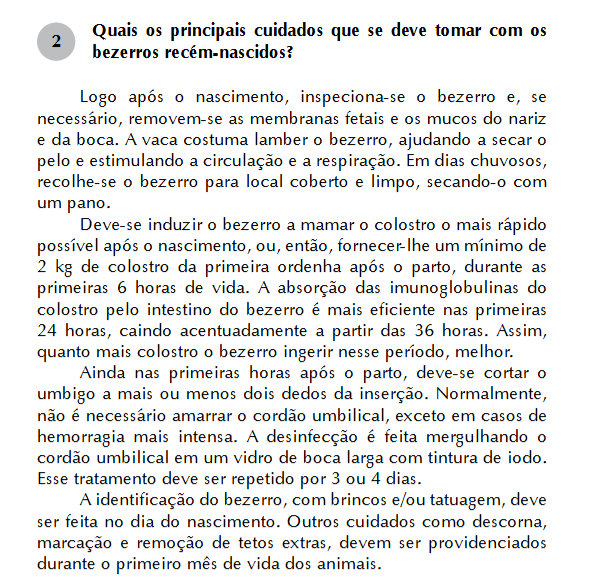
\includegraphics[width=0.60\linewidth]{imagens/ex_pergunta_livro.png}
    \caption{Exemplo de Pergunta: Fonte : \cite{embrapa2012gadoleite}}
    \label{fig:ex_pergunta_livro}
\end{figure}


\begin{table}[H]
    \centering
    \begin{tabularx}{\textwidth}{c|p{6cm}|>{\raggedright\arraybackslash}X}
        \textbf{Número} & \textbf{Pergunta} & \textbf{Resposta} \\
        \midrule
        2 & Quais os principais cuidados que se deve tomar com os bezerros recém-nascidos? & 
        Logo após o nascimento, inspeciona-se o bezerro e, se necessário, removem-se as membranas fetais e os mucos do nariz e da boca. A vaca costuma lamber o bezerro, ajudando a secar o pelo e estimulando a circulação e a respiração. Em dias chuvosos, recolhe-se o bezerro para local coberto e limpo, secando-o com um pano. Deve-se induzir o bezerro a mamar o colostro o mais rápido possível após o nascimento, ou, então, fornecer-lhe um mínimo de... \\
    \end{tabularx}
    \caption{Exemplo da coleta de Perguntas e Respostas do livro "500 Perguntas e Respostas sobre Gado de Leite" em CSV.}
    \label{tab:exemplo_livro_csv}
\end{table}



Esse processo contribuiu para uma maior eficácia e consistência dos dados, os quais serão utilizados na formulação das respostas pelos modelos, uma vez que essas informações influenciam diretamente o desempenho dos algoritmos na etapa de aprendizado.

\section{Mineração de Dados}
A etapa de Mineração de Dados teve como objetivo analisar e comparar o desempenho das estratégias de geração de respostas no domínio da pecuária leiteira. Inicialmente, foi utilizada a configuração com prompts \textit{Zero-shot} como linha de base. Posteriormente, essa abordagem foi comparada a sistemas baseados em RAG, alimentados com documentos específicos da área leiteira. O propósito foi verificar se há diferença significativa na qualidade das respostas geradas, avaliando em que medida a incorporação de informações contextuais contribui para o aprimoramento da geração no domínio estudado.

\subsection{Zero-shot}

O \textit{Zero-shot}, conforme descrito por \cite{zero-shot}, também é conhecido como instrução de tarefa. Ele consiste em formular um prompt que forneça uma descrição formal e detalhada da tarefa a ser realizada. Na Figura \ref{fig:Representação Zero-shot}, apresentamos o prompt utilizado neste projeto.

O \textit{Zero-shot} foi aplicado em duas APIs de modelos de linguagem: 

\begin{itemize}
    \item \textbf{API GPT (OpenAI)} \cite{openai2023chatgpt}: Disponibiliza modelos como GPT-3 e GPT-4, capazes de gerar respostas complexas e coerentes a partir de prompts detalhados.
    \item \textbf{API LLAMA (GroqAPI)} \cite{touvron2023llamaopenefficientfoundation}: Oferece modelos LLM gratuitos, como LLAMA-3.1, LLAMA-3.3 e LLAMA-8b, focados em tarefas de linguagem com boa performance para instruções específicas.
\end{itemize}

\begin{figure}[H]
    \centering
    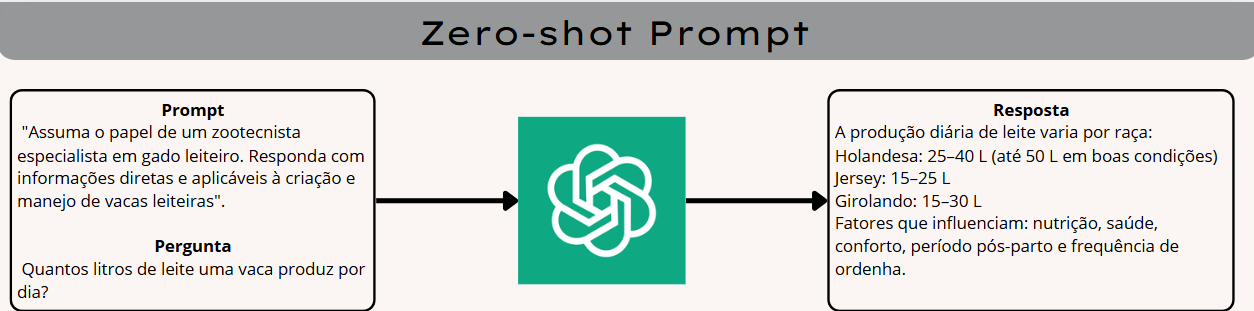
\includegraphics[width=1.0\linewidth]{imagens/zeroshot.png}
    \caption{Exemplo de Zero-shot. Fonte: Elaboração Própria}
    \label{fig:Representação Zero-shot}
\end{figure}

Como ilustrado na Figura \ref{fig:Representação Zero-shot}, o prompt define a tarefa a ser realizada e, junto da pergunta do usuário, é enviado ao modelo. Com base nesse contexto, o modelo gera a resposta mais adequada à tarefa, sem receber exemplos prévios.

    
\subsection{\textit{Few-shot}}

O \textit{Few-shot} difere do Zero-shot ao fornecer algumas demonstrações da tarefa durante a inferência, servindo como condicionamento para que o modelo execute a tarefa sem necessidade de atualização de pesos \cite{brown2020languagemodelsfewshotlearners}. Dessa forma, utiliza-se os exemplos fornecidos para que o modelo aprenda os padrões e estruture a resposta de forma adequada.

Essa estratégia apresenta algumas vantagens, como o aproveitamento de modelos pré-treinados e a fácil adaptação a novas tarefas. Entretanto, também possui desvantagens: requer, mesmo que em pequena quantidade, dados específicos para definir a tarefa e, geralmente, apresenta resultados inferiores aos de modelos ajustados por RAG, que utilizam informações do documento para contextualizar a resposta, resultando em uma resposta mais completa e fonte de dados verificável.

\begin{figure}[H]
\centering
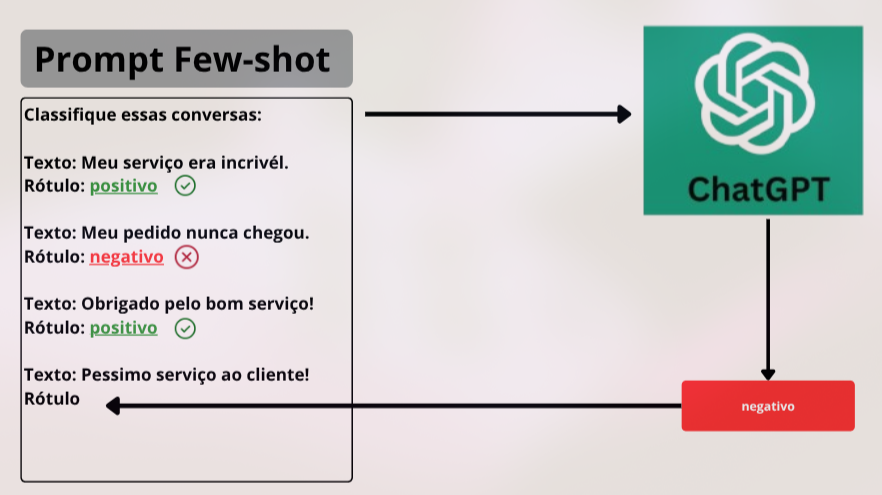
\includegraphics[width=0.75\linewidth]{imagens/few_shot1.png}
\caption{Representação adaptada e traduzida do Few-shot. Fonte: \cite{few-shotPromptImage}}
\label{fig:Representação Few-shot}
\end{figure}

A Figura \ref{fig:Representação Few-shot} demonstra o uso do \textit{Few-shot} na tarefa de classificar conversas quanto ao teor positivo ou negativo. Para isso, são fornecidos três exemplos de conversas acompanhados de suas classificações esperadas. Em seguida, apresenta-se um novo texto para que o modelo aplique a mesma tarefa. Com base no contexto fornecido pelos exemplos, o modelo analisa o texto em busca de padrões que permitam identificar a classe à qual ele pertence.

No presente trabalho, o Few-shot foi empregado como recurso complementar na construção dos prompts das abordagens baseadas em RAG, não sendo avaliado de forma isolada.

\subsection{RAG}

    O RAG é uma técnica que busca aprimorar a geração de respostas de modelos de LLM por meio do fornecimento de uma base de dados externa, como apontado por \cite{lewis2021retrievalaugmentedgenerationknowledgeintensivenlp}, a qual demonstra que esses modelos possuem limitações em tarefas que exigem conhecimento específico, atualizado ou explicações detalhadas.

    Nesse contexto, o RAG surge como uma solução para essas limitações, permitindo o uso de conhecimento proprietário. Documentos e artigos que não podem ser compartilhados publicamente, como e-mails, documentos internos e relatórios, podem ser utilizados como dados para a geração de respostas, proporcionando um contexto específico sobre o funcionamento da instituição, onde será aplicado. Além disso, o modelo pode citar fontes reais e atuais, mostrando de forma transparente a origem das informações utilizadas na geração da resposta, aumentando a veracidade dos dados e facilitando a verificação dos fatos pelo usuário.


\begin{figure}[H]
    \centering
    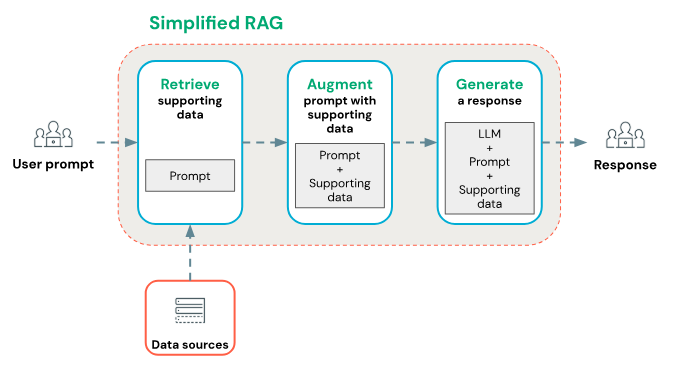
\includegraphics[width=0.8\linewidth]{imagens/representacao_rag.png}
    \caption{Representação do Funcionamento do RAG Fonte: \cite{microsoftRAG} }
    \label{fig:Representação RAG}
\end{figure}

Como descrito na Figura \ref{fig:Representação RAG}, o \textit{prompt} do usuário passa por três etapas, cada uma responsável por uma operação específica. A primeira etapa é a Recuperação, que analisa o \textit{prompt} e realiza a busca na base de dados externa, retornando informações de suporte que serão usadas como contexto adicional. Em seguida, ocorre a etapa de Aumentação, que combina os dados de suporte com o \textit{prompt} do usuário, gerando um \textit{prompt} mais contextualizado e relevante. Por fim, o \textit{prompt} aumentado é enviado ao modelo, permitindo a geração de respostas mais detalhadas e precisas, alinhadas com os dados de suporte.



Com isso foi estudamos 2 ferramentas que permitem realizar a tarefa de RAG:



\subsection{LightRAG}
LightRAG é um novo framework para aprimoramento de modelos de LLM por meio de RAG. Proposto por \cite{LightRag}, ele busca suprir duas principais limitações presentes nos sistemas de RAG tradicionais. A primeira delas é que muitos métodos dependem de representações planas, o que restringe a capacidade de compreender e recuperar informações baseadas nas relações entre entidades. A segunda limitação refere-se à lacuna de contexto, frequentemente insuficiente para manter a coerência entre diversas entidades, o que pode resultar em respostas que não atendem plenamente à consulta do usuário.

Para superar esses desafios, o LightRAG adota uma estratégia de recuperação em dois níveis, aprimorando a capacidade de compreensão e recuperação de informações tanto no nível inferior, voltado para a precisão e o detalhamento de entidades e seus relacionamentos, enquando o no nível superior, que abrange temas mais amplos e favorece a descoberta de conhecimento de forma contextualizada.

Além disso, o LightRAG incorpora estruturas de grafos no processo de indexação e recuperação de informações. A representação por meio de grafos facilita a modelagem eficaz das inter-relações entre entidades, permitindo uma recuperação de informação mais precisa e contextualizada.


Com essas abordagens, os autores alcançam maior efetividade e eficiência no sistema de RAG ao resolver três pontos cruciais, a Recuperação de Informação Compreensiva, garantindo a coleta completa do contexto e das interdependências entre entidades ao longo dos documentos. Posteriormente, a melhora na eficiência de recuperação, por meio da exploração da estrutura de conhecimento em grafos, o que reduz significativamente o tempo de resposta. Por ultimo a rápida adaptação a novos dados, permitindo que o sistema se ajuste rapidamente a atualizações, mantendo sua relevância em ambientes dinâmicos.

\subsubsection{Geração de Grafico}

\begin{figure}[H]
    \centering
    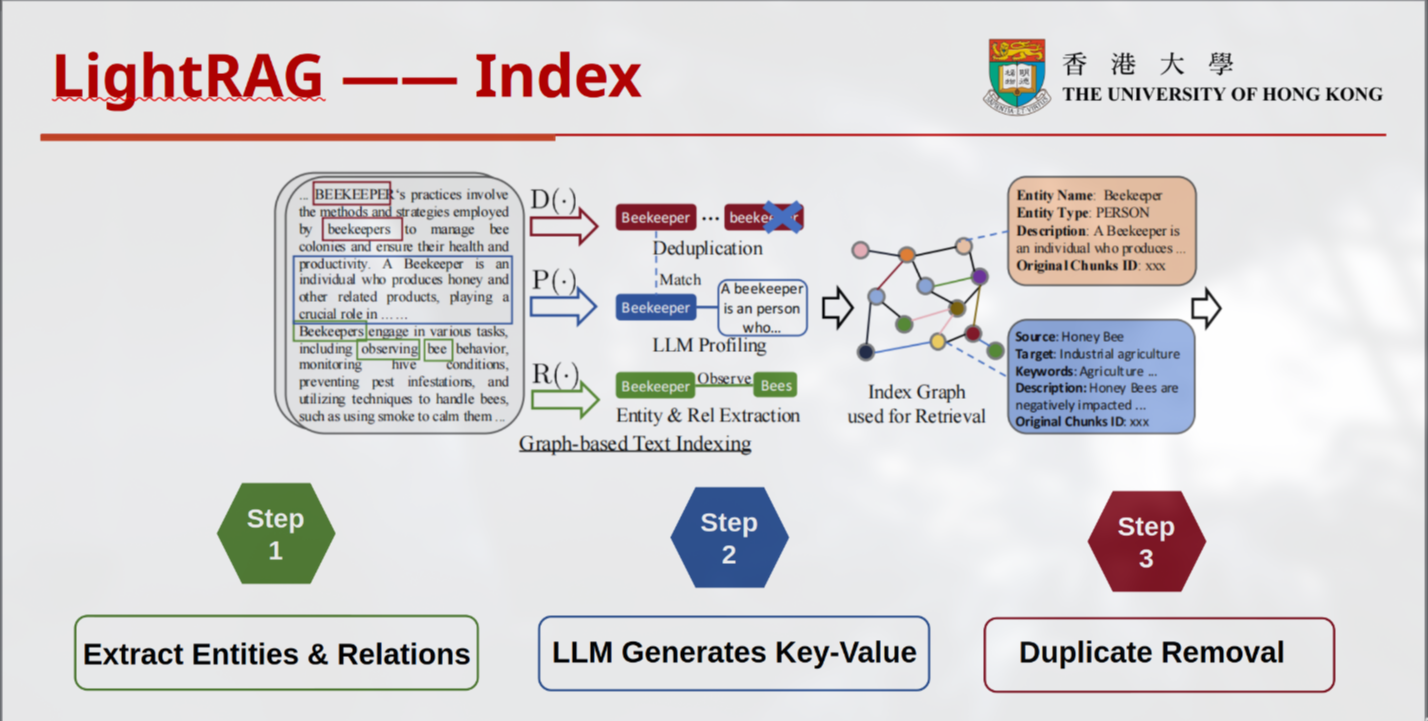
\includegraphics[width=1.0\linewidth]{image.png}
    \caption{Representação da Etapa de Indexação das informações no formato de gráfico. Fonte: \cite{LightRag}}
    \label{fig:light_rag_representation}
\end{figure}


A Figura \ref{fig:light_rag_representation} ilustra o fluxo de indexação e recuperação de conhecimentos no sistema. Inicialmente, documentos e dados brutos atravessam um pipeline dedicado à extração de entidades para a criação de nós e arestas para a criação e expansão do gráfico de conhecimento. Os nós armazenam as descrições das entidades, enquanto as arestas representam as relações semânticas com as demais entidades do gráfico, permitindo uma busca baseada na similaridade com a consulta do usuário.

O cálculo que representa a criação do Gráfo de conhecimento se dá pela formula \ref{eq:light_rag_graph_generation}

\begin{equation}
\label{eq:light_rag_graph_generation}
    \hat{D} = (\hat{V}, \hat{E}) = \text{Dedupe} \circ \text{Prof}(V, E), \quad \text{onde } V, E = \bigcup_{D_i \in D} \text{Recog}(D_i)
\end{equation}

Onde:
\begin{itemize}
    \item \( \hat{D}\): Grafo de Conhecimento;
    \item \( \hat{V}\):  Vértices do Grafo de Conhecimento;
    \item \( \hat{Ê}\): Arestas do Gráfo de Conhecimento;
    \item \(D \): Refêrente ao corpo do texto (Banco de Dados externo);
    \item \(D_i \): São as \textit{chunks} (segmentos) dos texto;
    \item \(Recog\): Função de Extração de Entidades e Relacionamentos;
    \item \(Prof\):  Função de Profilamento, usa um LLM para fazer a extração de chave-valor para a entidades e relacionamentos;
    \item \(Dedupe\): Função de Deduplicação, que faz a mesclagem de entidades repetidas;



\end{itemize}

Neste processo, cada função desempenha um papel específico. A primeira delas é o Recon (Reconhecimento), responsável pela extração de entidades e relacionamentos a partir de segmentos de texto. Utilizando um LLM, esta função analisa cada segmento isoladamente. Posteriormente, os resultados obtidos de todos os segmentos são unificados. Viabilizando a geração de um grafo de conhecimento, onde as conexões representadas de forma estruturada.

A segunda etapa é o Prof (Profilamento), responsável pela criação de chaves para cada entidade e relacionamento, visando facilitar o processo de recuperação. Nesta fase, um LLM é aplicado sobre o conjunto de segmentos para gerar pares chave-valor: as chaves garantem uma recuperação eficiente, enquanto os valores contêm parágrafos que resumem os trechos relevantes.

Por fim, na terceira etapa, atua o Dedupe (Deduplicação), responsável por identificar e unificar entidades e relacionamentos duplicados extraídos de diferentes segmentos. Esta etapa é crucial para otimizar o grafo, reduzindo seu tamanho ao eliminar redundâncias, mantendo apenas informações únicas e consolidando dados complementares.




\begin{figure}[H]
    \centering
    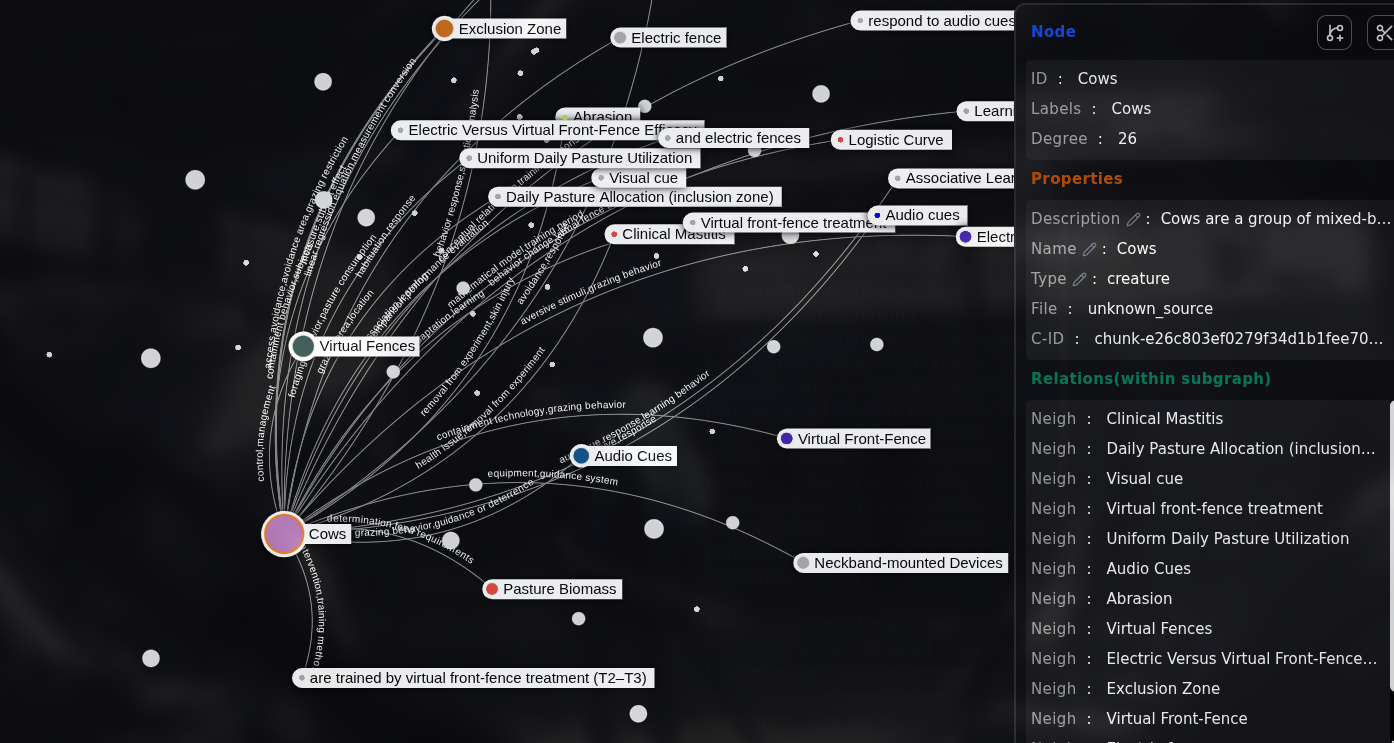
\includegraphics[width=1.0 \linewidth]{imagens/light_rag-representacao_grafo.png}
    \caption{Representação do Grafo de Conhecimento. Fonte: Elaboração Própria}
    \label{fig:light_rag-representacao_grafo}
\end{figure}

Finalizado o processo de indexação, obtém-se um Grafo de Conhecimento que consolida as propriedades das entidades descobertas, os documentos de origem e, fundamentalmente, as relações semânticas entre os elementos, como referenciado pela figura \ref{fig:light_rag-representacao_grafo}. A recuperação de informações ocorre por meio da navegação nesse grafo, onde a consulta do usuário é decomposta em conceitos de baixo nível \textit{(Low-Level Keys)} e conceitos abrangentes \textit{(High-Level Keys)}. O sistema realiza uma busca transversal em todos os nós correlacionados, retornando os trechos específicos de onde as informações foram extraídas. Esse fluxo fornece um contexto enriquecido e estruturado, permitindo que o modelo de linguagem gere respostas com maior precisão e fundamentação teórica.


\subsection{Geração de Resposta}

O processo de geração de resposta no sistema LightRAG inicia-se com a decomposição da consulta do usuário em dois níveis de granularidade: conceitos específicos e temas abrangentes. O prompt de instrução responsável por essa extração está representado na Figura \ref{fig:light_rag-prompt_extração de keywords}.


\begin{figure}[H]
    \centering
    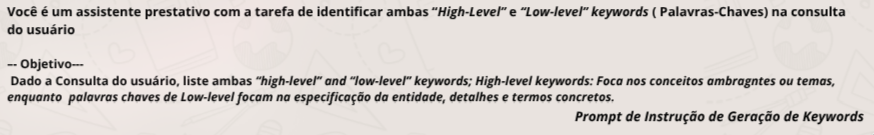
\includegraphics[width=1\linewidth]{imagens/light_rag-prompt_de_instrucao_extracao_de_keywords.png}
    \caption{Prompt de Instrução de Geração de Keywords. Fonte: Elaboração Própria}
    \label{fig:light_rag-prompt_extração de keywords}
\end{figure}

Para assegurar a consistência e o formato das saídas, utiliza-se a técnica de \textit{Few-shot}, cujo propósito é estabelecer um padrão de resposta esperado por meio da demonstração de exemplos práticos, conforme ilustrado na Figura \ref{fig:ligth_rag-prompt_geracao_de_entrada_de_keywords}.

\begin{figure}[H]
    \centering
    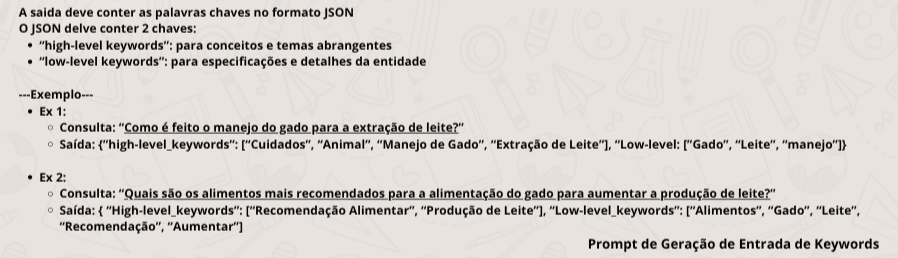
\includegraphics[width=1\linewidth]{ligth_rag-prompt_geracao_de_entrada_de_keywords.png}
    \caption{Prompt de Geração de Entrada de Keywords. Fonte: Elaboração Própria}
    \label{fig:ligth_rag-prompt_geracao_de_entrada_de_keywords}
\end{figure}


Uma vez extraídas as palavras-chave, o sistema realiza a navegação no grafo de conhecimento. A aplicação desse fluxo sobre a consulta original permite que o motor de busca identifique e recupere as entidades e relações mais relevantes, consolidando um contexto técnico enriquecido (Figura \ref{fig:light_rag-recuperacao_de_contexto}). Esse mecanismo mitiga a lacuna de contexto comum em sistemas tradicionais, resultando em uma resposta final mais completa e assertiva (Figura \ref{fig:light_rag-resposta_gerada}).

\begin{figure}[H]
    \centering
    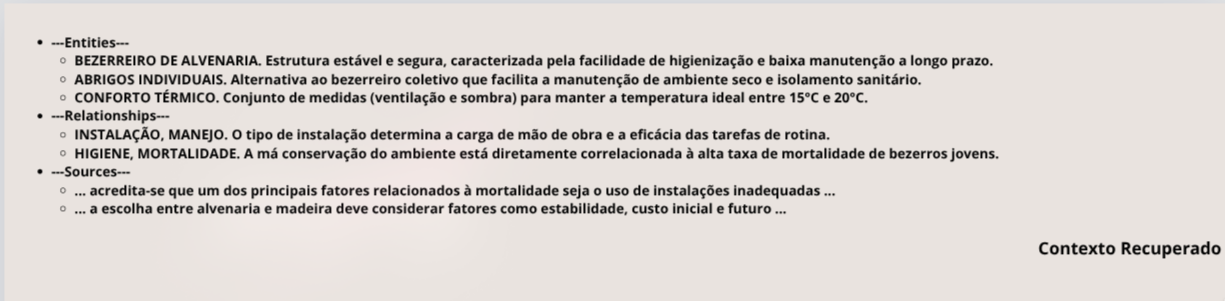
\includegraphics[width=1\linewidth]{imagens/light_rag-recuperacao_de_contexto.png}
    \caption{Contexto Recuperado pelo Ligth RAG. Fonte: Elaboração Própria}
    \label{fig:light_rag-recuperacao_de_contexto}
\end{figure}

\begin{figure}[H]
    \centering
    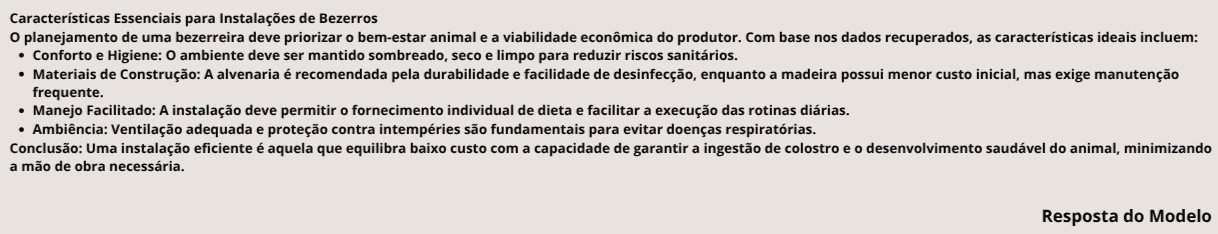
\includegraphics[width=1\linewidth]{imagens/light_rag-resposta_gerada1.png}
    \caption{Resposta Gerada pelo Ligth RAG. Fonte: Elaboração Própria}
    \label{fig:light_rag-resposta_gerada}
\end{figure}

\section{G-RAG-LiveRAG}
O G-RAG (ou LiveRAG) foi o sistema vencedor do desafio LiveRAG na conferência SIGIR 2025 (\textit{Special Interest Group on Information Retrieval}). A arquitetura propõe uma abordagem de Geração de Recuperação Aumentada baseada na criação de respostas hipotéticas para a consulta original do usuário. O objetivo central é o enriquecimento do vocabulário e do contexto semântico de perguntas que, rotineiramente, apresentam-se de forma excessivamente objetiva, como: "Qual vaca produz mais leite?".

Assim, o modelo gera uma resposta hípotetica imprecisas, como atribuir a maior produção à raça Jersey em vez da Holandesa, expandindo o vetor da consulta. Ao realizar a combinação da pergunta original com a resposta hipotética, o sistema amplia o argumento de busca, otimizando a relação semântica entre a consulta e os chunks de documentos indexados. Essa técnica eleva a taxa de recuperação de informações pertinentes, permitindo que a resposta final seja mais robusta e abranja conhecimentos que a pergunta simplista do usuário, isoladamente, não seria capaz de extrair da base de dados.

\subsection{Fluxo de Execução}

\begin{figure}[h]
    \centering
    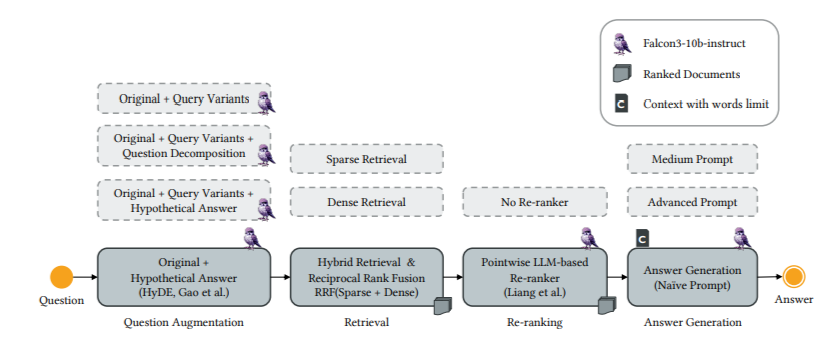
\includegraphics[width=1\linewidth]{imagens/fluxo_g_rag.png}
    \caption{Fluxo de geração de resposta do G-RAG, Fonte: \cite{G-RAG-LiveRAG}}
    \label{fig:g-rag-fluxo_de_trabalho}
\end{figure}

Ao passar a pergunta para o modelo, chega-se à primeira etapa do sistema, que consiste em aumentar a consulta original por meio de três técnicas possíveis, visando ampliar o contexto da dúvida do usuário e auxiliar o modelo a encontrar documentos que forneçam subsídios para uma resposta mais precisa. Esses documentos são selecionados com base na semelhança entre os termos presentes na resposta gerada e o conteúdo do acervo. Entre as estratégias disponíveis, destaca-se a Variação de Consultas \textit{(Query Variants)}, na qual definem-se $k$ variações da pergunta original para serem utilizadas como consultas de busca. Outra abordagem é a Consulta de Decomposição, que realiza diversas chamadas ao LLM para desmembrar a pergunta em subconsultas até identificar seu significado essencial, utilizando-o para reformular a questão original com detalhes mais importantes. Por fim, a Geração de Resposta Hipotética \textit{(Hypothetical Answer Generation)} permite que um modelo mais leve responda à pergunta inicial com maior flexibilidade. Embora essa resposta possa ser apenas parcialmente correta, ela cumpre o papel fundamental de servir como um contexto expandido de busca durante a etapa subsequente de recuperação.

Com a pergunta aumentada, passamos para a etapa de recuperação híbrida, composta por 2 tipos de recuperação,  a Esparsa, a qual busca por documentos que tenha a correspondencia exata das palavras chaves e entidades únicas contida na pergunta aumentada e a Recuperação Densa, faz a recuperação focada na semântica, retornando documentos que apresentem mesmas palavras ou significados semelhantes, utilizando a semelhança do cosseno para fazer essa comparação, dados todos os documentos recuperados, e aplicado o \textit{Reciprocal Rank Fusion} (RRF), para unir os 2 resultados obtidos por cada método é retorna apenas os documentos mais relevantes para a geração da resposta.

Com a lista de documentos relevantes para a pergunta partimos, passamos por um re ranqueamentos dos documentos obtidos na etapa anterior e passamos para um modelo de ponta avaliar, para verificar se os documentos contém informação necessária para responder a pergunta. Onde são rankeados pela taxa de semelhança, e caso a semelhança for inferior a 0.5, o documento e descartado. Posteriormente, para a geração da resposta final, passamos um prompt de instrução para o modelo descrevendo a tarefa a ser realizada pelo modelo, em conjunto dos documentos relevantes e o prompt aumentado, assim aprimorando a resposta gerada pelo modelo com prompt mais robusto e documentos relevantes.


\section{Avaliação do Modelo}
Para avaliar a qualidade das respostas geradas, foram utilizadas métricas amplamente difundidas na área de Processamento de Linguagem Natural, que comparam o texto de referência com o texto produzido pelo modelo. Além disso, foi aplicado o teste estatístico t-test como critério de desempate entre modelos que apresentaram resultados semelhantes. A função do t-test é verificar se a diferença entre as médias é estatisticamente significativa. Considerando um nível de significância de 5\%, quando o valor de \textbf{p} > 0{,}05, entende-se que não há diferença estatisticamente significativa entre os modelos; quando \textbf{p} < 0{,}05, pode-se assumir que há diferença significativa entre os desempenhos comparados. O teste foi aplicado considerando as médias das métricas obtidas em cada conjunto de respostas.



\subsection{BERTScore:}
O BERTScore é uma metrica de avaliação que busca fazer a comparação dado as sentenças de referência com uma sentença gerada, utilizando representações contextuais em forma de embeddings. A ideia central é calcular a taxa de correspondencia semantica entre os textos por meio da similidaridade do cosseno entre os vetores obtidos, como descrito por \cite{zhang2020bertscoreevaluatingtextgeneration}

\begin{figure}[H]
    \centering
    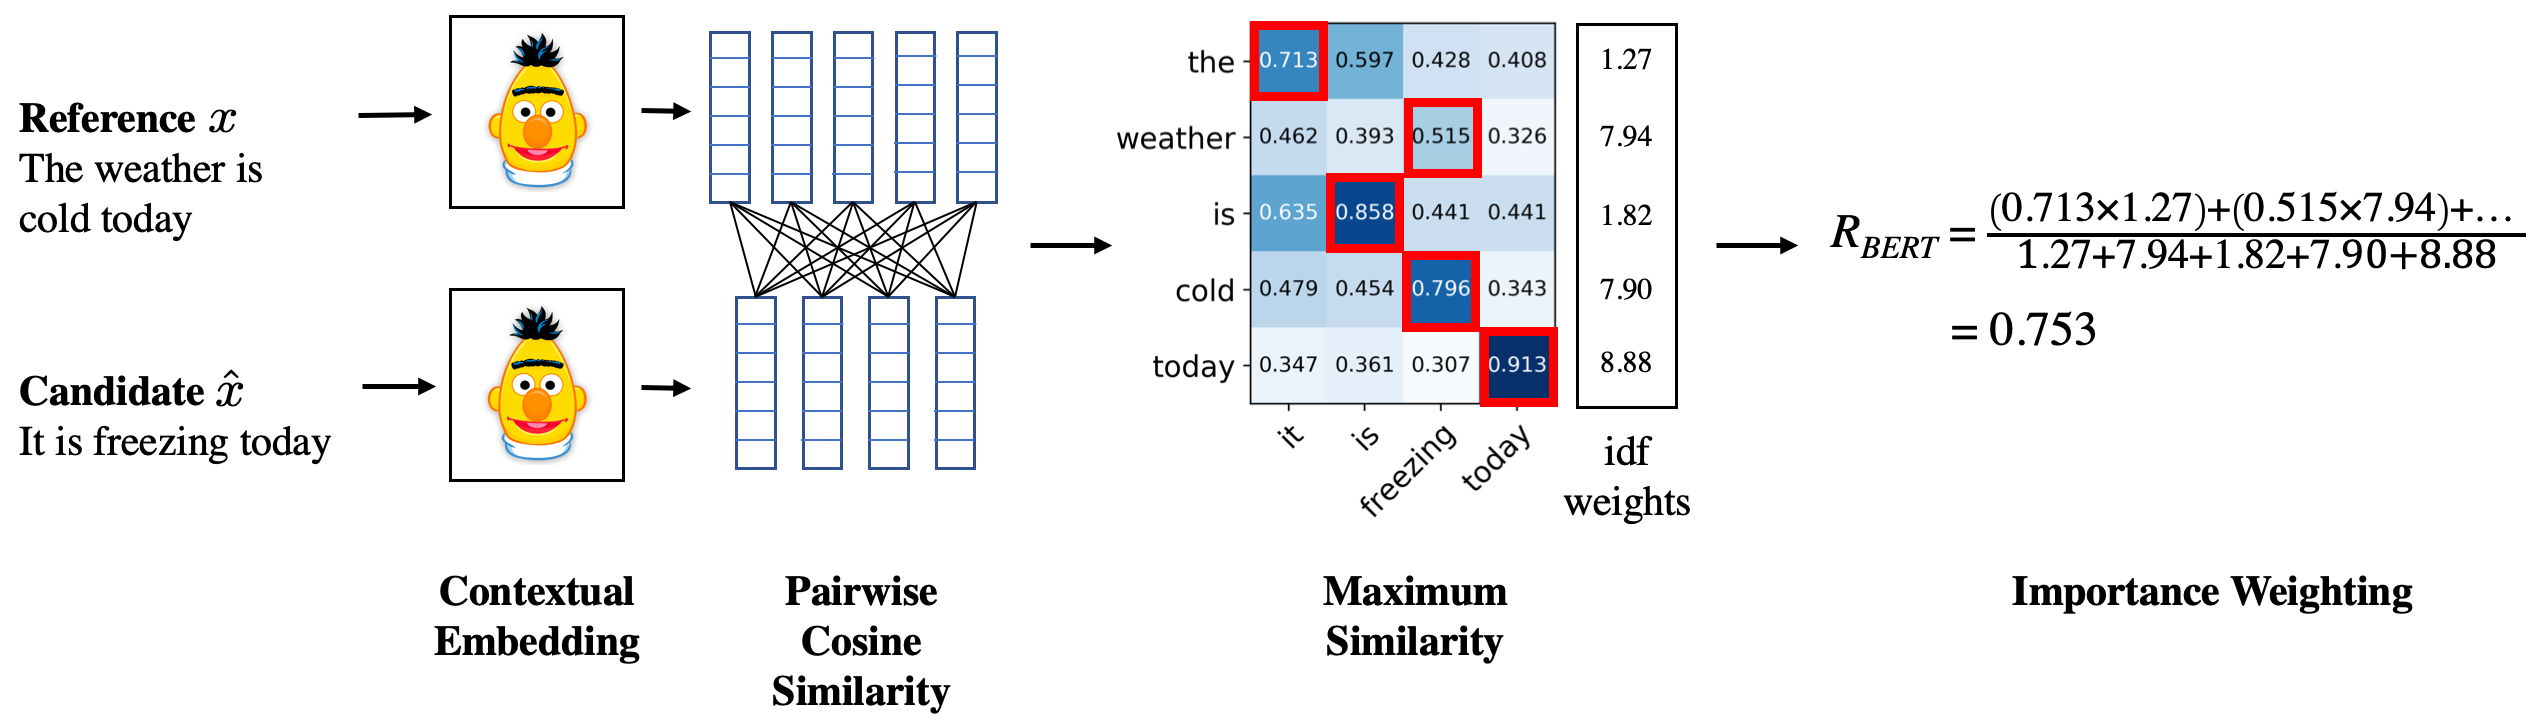
\includegraphics[width=0.8\linewidth]{imagens/bartscore.png}
    \caption{Ilustração do cálculo de recall $R_{BERT}$ Fonte:\cite{zhang2020bertscoreevaluatingtextgeneration}}
    \label{fig:bertscore_representation}
\end{figure}

O pipeline descrito na Figura \ref{fig:bertscore_representation} representa o processo executado pelo BERT, que consiste na conversão dos textos em vetores de embeddings contextuais, obtidos a partir das camadas do modelo BERT selecionado. Onde, posteriormente, é calculada a similaridade do cosseno, de modo a identificar as palavras que apresentam maior semelhança semântica entre os textos.


Possibilitando realizar a análise em ambos os sentidos: na precisão \ref{eq;precisonBert}, que mede o grau de correspondência semântica das palavras da sentença candidata em relação à referência e no recall \ref{eq;recallBert}, que avalia em que medida as palavras da referência encontram correspondência semântica na sentença candidata. Ao calcular a média harmônica entre os valores de precisão e recall \ref{eq;F1Bert}, obtém-se um equilíbrio entre as duas métricas, capturando de forma mais robusta a similaridade entre os textos.

\begin{equation}
\label{eq;precisonBert}
    P_{\text{BERT}} = \frac{1}{|y|} \sum_{y_j \in y} \max_{x_i \in x} (x_i^\top y_j)
\end{equation}

\begin{equation}
\label{eq;recallBert}
    R_{\text{BERT}} = \frac{1}{|x|} \sum_{x_i \in x} \max_{y_j \in y} (x_i^\top y_j)
\end{equation}

\begin{equation}
\label{eq;F1Bert}
    F_{BERT} = 2 \frac{P_{BERT} * R_{BERT}}{P_{BERT} + R_{BERT}}
\end{equation}


Onde:
\begin{itemize}
    \item \(x\): Conjunto de Embeddings das palavras do Texto Gerado.
    \item \(y\):  Conjunto de Embeddings das palavras do Texto Referência
    \item \(x_iT y_j\): Similaridade do Cosseno entre os embeddings do token candidato \(x_i\) e o embeddings do token de referência \(y_j\).
\end{itemize}

\subsubsection*{Exemplo do BERTScore}

Considere a sentença de referência:

\begin{itemize}
    \item \textbf{Referência}: \textit{``A vaca produz de 15 a 30 litros de leite todos os dias.''}
\end{itemize}

E duas sentenças geradas:

\begin{itemize}
    \item \textbf{Texto Gerado 1}: \textit{``A vaca dá entre 15 e 30 litros de leite diariamente.''}
    \item \textbf{Texto Gerado 2}: \textit{``A vaca come muito capim todos os dias.''}
\end{itemize}

O BERTScore converte cada palavra em representações vetoriais contextuais (embeddings) e calcula a similaridade do cosseno entre as palavras da referência e as da sentença candidata. Dessa forma, é possível capturar semelhanças semânticas mesmo quando há variações lexicais. 

A Tabela \ref{tab:exemplo_bertscore} mostra valores ilustrativos de precisão, recall e F1 do BERTScore para os dois textos gerados:

\begin{table}[H]
    \centering
    \begin{tabular}{lccc}
        \toprule
        \textbf{Sentença} & \textbf{Precisão ($P_{BERT}$)} & \textbf{Recall ($R_{BERT}$)} & \textbf{F1 ($F_{BERT}$)} \\
        \midrule
        Texto Gerado 1 & 0.94 & 0.93 & 0.935 \\
        Texto Gerado 2 & 0.41 & 0.39 & 0.40 \\
        \bottomrule
    \end{tabular}
    \caption{Exemplo de cálculo do BERTScore para duas sentenças geradas.}
    \label{tab:exemplo_bertscore}
\end{table}

Observa-se que o \textbf{Texto Gerado 1} obteve uma pontuação elevada, indicando alta similaridade semântica com a referência, mesmo utilizando palavras diferentes (\textit{``produz''} $\approx$ \textit{``dá''}, \textit{``todos os dias''} $\approx$ \textit{``diariamente''}). Já o \textbf{Texto Gerado 2} obteve valores baixos, pois apesar de compartilhar o contexto de ``todos os dias'', não preserva a informação central sobre a produção de leite.


\subsection{BARTScore:}
BARTScore é uma metrica de avaliação de textos gerados por LLMs, diferentemente do BERTScore, essa métrica não faz uso da similidaridade vetorial, mas sim da similariedade logarítimica, de que dado um texto base, o modelo BART é capaz de repoduzir a mesma saída, apartir do texto de referência \cite{NEURIPS2021_e4d2b6e6}, seguindo a Equação \ref{eq:BartScore}.
\newline

\textbf{Fórmula do BARTScore:}
\begin{equation}
    \label{eq:BartScore}
    BARTScore(x, y) = \sum_{t=1}^{m} w_t \log p(y_t \mid y_{<t}, x,\theta)
\end{equation}

Onde:
\begin{itemize}
    \item \(m\): Tamanho da sequência de saída
    \item \(w_t\): Pesos atribuido a cada token
    \item \(y_t\): Token na posição de saída
    \item \(x\): Texto de entrada
    \item \(\theta\): Parâmetros do modelo BART utilzado

\end{itemize}


\textbf{Exemplo}:

\begin{table}[H]
\resizebox{\linewidth}{!}{%
\begin{tabular}{|c|c|c|}
\hline
Texto Referência & Texto Candidato  & BARTScore \\
\hline
A vaca produz de 15 a 30 litros de leite todos os dias & A produção de laticínios por vacas é de aproximadamente 15 a 30 litros por dia & -0.43\\
A alimentação é um fator que influência diretamente na saúde do animal & Como realizar o controle de moscas do meio rural & -4.02 \\

\hline

\end{tabular}
}
\caption{Exemplo do cálculo do BartScore}
\label{tab:exemploBart}
\end{table}

Na Tabela \ref{tab:exemploBart}, para textos que apresentam uma alta taxa de semelhança semântica, eles recebem scores altos (valores menos negativos) e para texto considerados diferentes, apresentam scores mais baixos (mais negativos), indicando uma baixa relação semântica entre eles. 



\subsection{GPTScore:}
Como descrito por \cite{fu2023gptscoreevaluatedesire}, a métrica GPTScore baseia-se na utilização de um modelo GPT para atribuir uma probabilidade à geração de textos de alta qualidade, considerando como parâmetros a descrição da tarefa e a definição dos aspectos de avaliação. Para isso, é construído um prompt contendo a tarefa, os critérios de avaliação definidos e o contexto de entrada. Dado esse prompt, o modelo calcula a probabilidade de gerar o texto fornecido. Uma alta probabilidade indica que o texto está alinhado com o que o LLM “esperaria gerar”, dado o contexto e a tarefa, refletindo, assim, sua qualidade semântica e coerência.


\textbf{Fórmula do GPTScore:}

\begin{equation}
    GPTScore(h | d, a, S) = \sum_{t=1}^{m}w_t log p(h_t|h_{<t}, T(d,a,S), \theta)
\end{equation}

Onde:
\begin{itemize}
    \item \(h = (h1, h2, ..., hn)\): Textos a serem avaliados;
    \item \(w_t\): Peso do token na posição t;
    \item \(d\): Descrição da Tarefa; 
    \item \(a\): Aspectos a ser avaliado;
    \item \(S\): Texto fonte ou referência;
    \item \(T(d,a,S)\): Template do prompt que define o protocolo de avaliação. 
\end{itemize}

\textbf{Exemplo}:

\textbf{Texto de Referência} (S): "Vacas leiteiras podem produzir entre 15 a 30 litros por dia, dependendo da alimentação e cuidados."

\textbf{Tarefa} (d): "Classifique se a sentença gerada preserva as mesmas informarções do texto de referência."

\textbf{Aspecto} (a): "Corretude factual."

\textbf{Texto Candidato}(h):
\begin{itemize}
    \item 1. "As vacas produzem de 15 a 30 litros de leite diariamente."
    \item 2. "Vacas podem produzir até 50 litros de leite por dia."
\end{itemize}

\begin{table}[H]
    \centering
    \begin{tabular}{c|c|c|c}
         Tokens de h1     &   h1(log p) &  Tokens de h2    &     h2(log p)    \\
         
         \midrule
         
         As             &   -0.05     &   Vacas       &     -0.03       \\
         Vacas          &   -0.04     &   podem       &     -0.02       \\
         produzem       &   -0.03     &   produzir    &     -0.10       \\
         de             &   -0.02     &   até         &     -0.05       \\
         15             &   -0.01     &   50          &     -0.15       \\
         a              &   -0.01     &   litros      &     -0.01       \\
         30             &   -0.01     &   de          &     -0.01       \\
         litros         &   -0.02     &   leite       &     -0.02       \\
         de             &   -0.01     &   por         &     -0.01       \\ 
         leite          &   -0.03     &   dia         &     -0.03       \\
         diariamente    &   -0.02     &    -          &       -         \\
    
         \bottomrule
         
         \textbf{Soma}  &   -0.25     &       -       &      -0.34     \\
    \end{tabular}
    \caption{Exemplo do Cálculo de GPTScore}
    \label{tab:exemploGPTScore}
\end{table}

A Tabela \ref{tab:exemploGPTScore} apresenta as probabilidades logarítmicas atribuídas a cada token, considerando a definição da tarefa e os aspectos avaliados. Valores menos negativos indicam maior coerência do texto gerado em relação ao contexto de referência. No exemplo, o texto \textbf{h1} obteve um GPTScore mais alto, por manter consistência semântica e respeitar as informações do texto de referência. Em contraste, o texto \textbf{h2} recebeu um score inferior, pois afirmou que “vacas produzem até 50 litros de leite”, divergindo da referência, que estabelece o intervalo de 15 a 30 litros. Essa diferença evidencia como o GPTScore consegue penalizar incoerências factuais nos textos gerados.




\subsection{BLEU:} 
A métrica BLEU (Bilingual Evaluation Understudy — Assistente de Avaliação Bilíngue) foi uma das primeiras métricas propostas para avaliação de similaridade textual, como descrito em \cite{papineni-etal-2002-bleu}. A tarefa primária da técnica é comparar os n-gramas do texto candidato com os n-gramas do texto de referência, realizando a contagem das correspondências entre eles. Quanto maior a taxa de correspondências, melhor é considerado o candidato de tradução. O cálculo da métrica é representado por \ref{eq:BleuScore}:
\newline

\textbf{Fórmula da Métrica BLEU}

\begin{equation}
\label{eq:BleuScore}
    \text{BLEU} = BP \cdot \exp\left( \sum_{n=1}^{N} w_n \cdot \log p_n \right)
\end{equation}




Onde:
\begin{itemize}
    \item \(BP\) é o \textit{Brevity Penalty}:
    \begin{equation}
        BP =
        \begin{cases}
          1, & \text{se } c > r, \\[6pt]
          e^{\left(\tfrac{1-r}{c}\right)}, & \text{se } c \leq r.
        \end{cases}
\end{equation}
    \item \(c\)  Comprimento do texto candidato 
    \item \(r\) Comprimento do texto referência
    \item \(N\) Número de N gramas considerados
    \item \(p_n\) é a precisão para os \(n\)-gramas
    \item \(w_n\) é o peso atribuído a cada \(n\)-grama (1/N).
\end{itemize}


\textbf{Exemplo}:
\begin{itemize}
    \item Referência: "A vaca produz leite todos os dias."
    \item Texto gerado: "Vaca produz leite diariamente."
\end{itemize}


\begin{equation}
    p_1 = \frac{3}{4} = 0{,}75, \quad p_2 = \frac{2}{3} \approx 0{,}67, \quad BP = e^{\frac{1-7}{4}} \approx 0{,}47
\end{equation}

\begin{equation}
\label{eq:blue_ex}
    \text{BLEU} = 0{,}47 \times \exp\left(0{,}5 \log 0{,}75 + 0{,}5 \log 0{,}67\right) \approx 0{,}33
\end{equation}

O resultado obtido no exemplo \ref{eq:blue_ex} foi de aproximadamente $0{,}33$ indicando que, apesar de existir alguma sobreposição de palavras e expressões entre a frase gerada e a referência, a similaridade lexical ainda é limitada. Isso ocorre porque o BLEU não reconhece variações semânticas como sinônimos ou mudanças de ordem das palavras. No exemplo, embora ``diariamente'' seja um equivalente semântico de ``todos os dias'', a métrica penaliza a ausência de correspondência exata nos $n$-gramas.



\subsection{ROUGE-N:} 
ROUGE (Recall-Oriented Understudy for Gisting Evaluation) é um conjunto de métricas para avaliação da qualidade dos resumos \cite{lin-2004-rouge}. O objetivo do ROUGE é medir quanto do conteúdo do texto de referência aparece no texto gerado. Ao contrário do BLEU, que foca em precisão, a qual é a quantidade dos n-gramas da referência está contido no texto gerado, o ROUGE enfatiza o recall. Assim, o ROUGE é mais tolerante a variação da ordem das palavras e foca em analisar a informação essencial por inteiro, ao invés de exigir as mesmas palavras exatas. Representado pela formula \ref{eq:Rouge}


\textbf{Fórmula de ROUGE-N}

\begin{equation}
\text{ROUGE-N} =
\frac{
    \sum_{S \in \text{ReferenceSummaries}} \sum_{gram_n \in S} \text{Count}_{\text{match}}(gram_n)
}{
    \sum_{S \in \text{ReferenceSummaries}} \sum_{gram_n \in S} \text{Count}(gram_n)
}
\label{eq:Rouge}
\end{equation}

Onde:
\begin{itemize}
    \item \(\textit{ReferenceSummaries}\):  Conjunto de textos de referência
    \item \(\textit{\(n-gram\)}\): Sequência de N palavras consecutivas.
    \item \(\textit{Count}\) \(\textit{gram\_n}\): Quantidade de palavras n-gramas no texto de referência.
    \item \(Count_match(gram_n)\): Quantidade de n-gramas que aparece tanto na referência quanto no texto candidado
\end{itemize}

\textbf{Exemplo:}

Considere os seguintes textos:

\begin{itemize}
    \item Texto referência: "A vaca produz leite todos os dias."
    \item Texto gerado: "Vaca produz leite diariamente."
\end{itemize}

Os unigramas da referência são: \{A, vaca, produz, leite, todos, os, dias\}

Os unigramas do texto gerado são: \{Vaca, produz, leite, diariamente\}

A contagem dos unigramas da hipótese que aparecem na referência é 3: \{vaca, produz, leite\}

O total de unigramas na referência é 7.

Logo, o ROUGE-1 (recall) é calculado como:

\[
\text{ROUGE-1} = \frac{3}{7} \approx 0{,}429
\]

Esse valor indica que cerca de 42,9\% dos unigramas do texto de referência foram recuperados no texto gerado.

